\documentclass[a4paper]{article}
\usepackage{nips13submit_e,times}
\usepackage{tikz}
\usepackage[english]{babel}
\usepackage[utf8]{inputenc}
\usepackage{amsmath}
\usepackage{graphicx}
\usepackage[all]{xy}
\usepackage{caption}
\usepackage{subcaption}
\usepackage{setspace}
\onehalfspace
\usepackage{anysize}
 
\usepackage[affil-it]{authblk}
\usepackage{color}
\usepackage{float}
\usepackage{natbib}

\usepackage{pgfplots, pgfplotstable}
%\pgfplotsset{compat=newest}

\title{\bfseries{Modeling the spread of the Measles Virus\\ using two different approaches}}
\nipsfinalcopy
\author{Christos Petropoulos (10867104) \\ Paula Subías Beltrán (10867112)}
\affil{University of Amsterdam \\ Introduction to Computational Science}
\date{\today}

\begin{document}

%% PRESENTATION
\maketitle

%% ABSTRACT
\begin{abstract}
The measles virus causes an infection at the respiratory system. It is one of the most contagious viruses that exist today. Therefore, the society should be able to handle any possible future outbreak. The purpose of this project, is to model and simulate the spread of the measles virus in the city of Manila, the capital of Philippines, which could help us predict how the virus may behave in a future outbreak. Two different models are used for the simulation process, known as SEIR model and Agent-based model. A description of both of those models is given and a comparison of their results as well.
\end{abstract}

%% INTRODUCTION
\section{Introduction}
The spread rate of a virus that is transmitted by contact, mostly depends on the rate of connectivity among the entire population. Focusing on the diffusion of a virus in a country, requires to take into account all of the interactions within its population, including the people who may stay there temporary. For example, on this year, the United States is experiencing a record number of Measles cases. In order to understand what causes that, we may have to study the origin of the area that most of the cases occur, as a possible outbreak in that area, to which U.S citizens travel a lot, can directly contribute to an increase of Measles cases in the U.S. A country which is frequently visited by the U.S citizens, is the Philippines. This year, several cases of measles have been detected there. According to the World Health Organization (WHO), the first half of the year, almost $50,000$ suspected cases of measles occurred, including $16,743$ confirmed cases and $97$ measles deaths. Due to this increase of Measles cases in the Philippines, a significant increase of Measles cases has also been happening in the U.S. The purpose of this project is to try and simulate how a possible Measles outbreak could evolve in the capital of the Philippines: Manila.

Measles is a highly contagious respiratory disease caused by the measles virus. The measles virus spreads by direct contact with an infected person having a contact rate of $75\%-90\%$. Usually, the virus spreads via droplets of fluid from the person's respiratory tract. These droplets contain millions of virus particles that can infect another person, entering through the respiratory tract. The virus incubates for one to two weeks before symptoms appear. After a few more weeks, the infection usually subsides. In developed countries, measles is usually not a fatal disease. However, many of the developing countries still have a high mortality rate.

Measles epidemics occur when the virus spreads rapidly through a susceptible population. The most vulnerable people are the ones who are not vaccinated. The higher the percentage of un-vaccinated people, the more susceptible a population is to an epidemic. In this report we model the spread of the measles virus in a city from a developing country. In other words, the spreading takes place in a city with high percentage of un-vaccinated people. Consequently, the risk of having an epidemic is higher than in other areas. 

In order to analyze the spreading process of the virus, we are going to use an Agent-based model, similar to what it is proposed in the report of \cite{Egypt}. An Agent-based model can recreate the entire population and its dynamics through incorporating social structures and heterogeneous connectivity patterns. The report of \cite{Egypt} proposes a stochastic multi-agent model to mimic the daily person-to-person contact of people. Later on, we will introduce the assumptions on which our model is based. 

In the following report, we introduce and describe the SEIR model and the proposed Agent-based model; created for the purpose of simulating the spread of the Measles virus. Finally, an analysis of their simulation results and a comparison among them is also given.

%% SEIR MODEL
\section{SEIR model}
The model of which the SEIR model is based on is called the SIR model. The SIR model was created by W. O. Kermack and A. G. McKendrick in 1927. Since then, a lot of modifications of that model have been proposed, with the SEIR model being one of those. The SEIR model assumes that the population is fixed (there is no increase/decrease of the population during the spread of the disease).

In the SEIR model, the population is divided into four distinct classes or states: the susceptible (S), the exposed (E), the infectious (I) and the recovered (R). The SEIR model simulates the spread of a disease using a system of differential equations which mathematically describe the rate at which the disease spreads through the entire population of an area, categorizing each of the persons into one of the classes that were described above.
 \begin{align*}
  \frac{dS}{dt} &= \mu N - \mu S - \beta S I, \\
  \frac{dE}{dt} &= \beta \frac{I}{N} S - (\mu + a) E, \\
  \frac{dI}{dt} &= a E - (\gamma+\mu) I, \\
  \frac{dR}{dt} &= \gamma I - \mu R.
 \end{align*}

The SEIR model uses some parameters which are defined by the disease's properties and the population's features:
\begin{itemize}
\item $\beta$: the contact rate between a susceptible and an infected person.
\item $\gamma$: the rate at which the infected person recovers and becomes resistant to the virus. And $\gamma^{-1}$ is the typical time until recovery.
\item $\alpha$: the rate at which a person who has been exposed to the virus, becomes infected. And $a^{-1}$ is the average incubation period.
\item $\mu$: the natural mortality and birth rate.
\end{itemize}

In order to use the SEIR model, some proper values need to be assigned as the parameters of the model. The contact rate of the Measles virus is between $0.75$ and $0.9$. Therefore, a value of $0.9$ has been assigned to the $\beta$ parameter. Later on, an analysis of the effect of choosing $0.75$ instead of $0.9$ as the contact rate, is also given. In addition, it is known that the typical time until recovery is between $8$ and $12$ days. So, we have defined $\gamma = \frac{1}{10} = 0.1$. Moreover, the average incubation period is between $7$ and $21$ days. Thus, the proper value for $a$ is $a= \frac{1}{14} = 0.07$. Last but not least, for the purpose of simplifying the Agent-based Model, the parameter $\mu$ has been set to zero ($\mu=0$). Due to the fact that the amount of people in the SEIR model remains constant, it is considered that there are neither deaths nor births. 
 
%% AGENT BASED MODEL
\section{Agent-based model}
An agent-based model consists of autonomous agents, the kinds of interactions among them and the effects of those interactions in the whole system as well. The Agent-based model can recreate an entire population and its dynamics. Thus, it can simulate the diffusion of a virus taking into account the interactions between the people that share an environment. 

For the development of the Agent-based model, the following factors have to be considered:
\begin{itemize}
\item \textit{City}: the size of the population and how it is distributed throughout the city. Also, the number of big  facilities (hospitals, universities, etc.) and public areas (i.e., parks, shopping malls, etc.).
\item \textit{Traffic}: the traffic of a city and its transportation system can affect the commuting and thus, the frequency at which people contact each other during the day with the purpose of getting to their destination. Therefore, this parameter is a major factor for the spread of a disease in a city.
\item \textit{Behaviour}: the set of activities and rules which define the kind of interactions and actions that an agent can perform during the simulation.
\end{itemize} 

\subsection{Modeling Manila}
In order to define the traffic around the city of Manila, we have used the transit map of it, which can been seen below in Figure (\ref{fig:map}). Due to the fact that we perform a small-scale simulation (simulating a population of $10,000$ people instead of the $1,652,171$ people that live in the city of Manila), we have decided to split the city into eight main areas. A graph representation of it can been seen below on (\ref{fig:map model}).

% Figure: model Manila
\begin{figure}[H]
\centering
\begin{subfigure}[b]{0.3\textwidth} 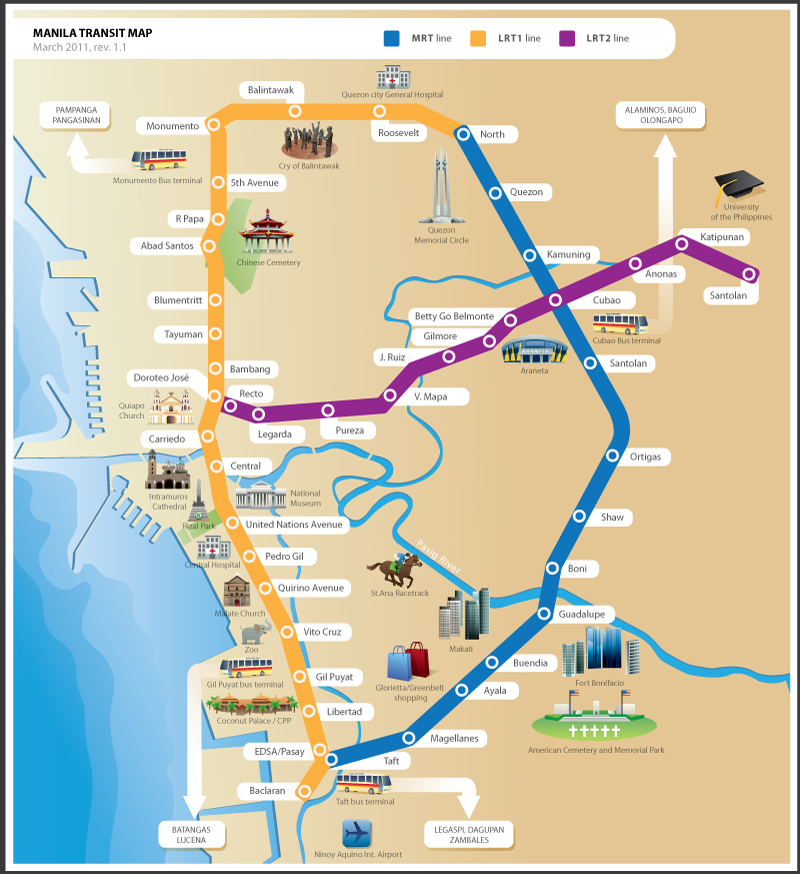
\includegraphics[width=\textwidth]{Manila-map}
\caption{Manila transit map (credits go to http://www.roomrent.ph/).}
\label{fig:map}
\end{subfigure} \quad     
\begin{subfigure}[b]{0.3\textwidth}
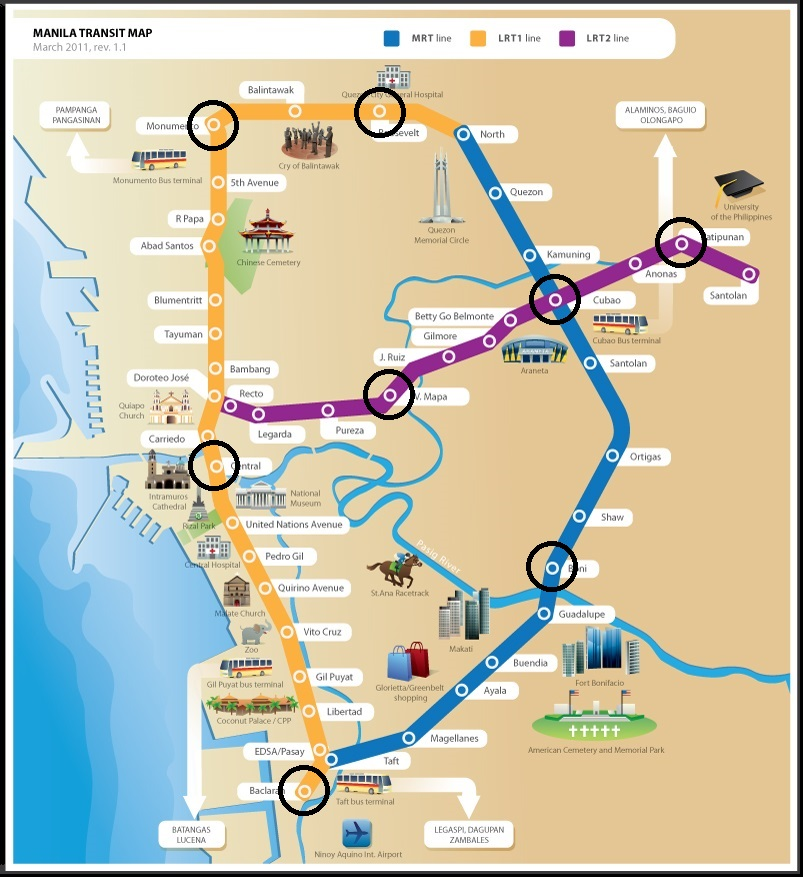
\includegraphics[width=\textwidth]{Manila-model_1}
\caption{Sketch of the nodes at the transit map.}
\label{fig:sketch map}
\end{subfigure} \quad
\begin{subfigure}[b]{0.3\textwidth}
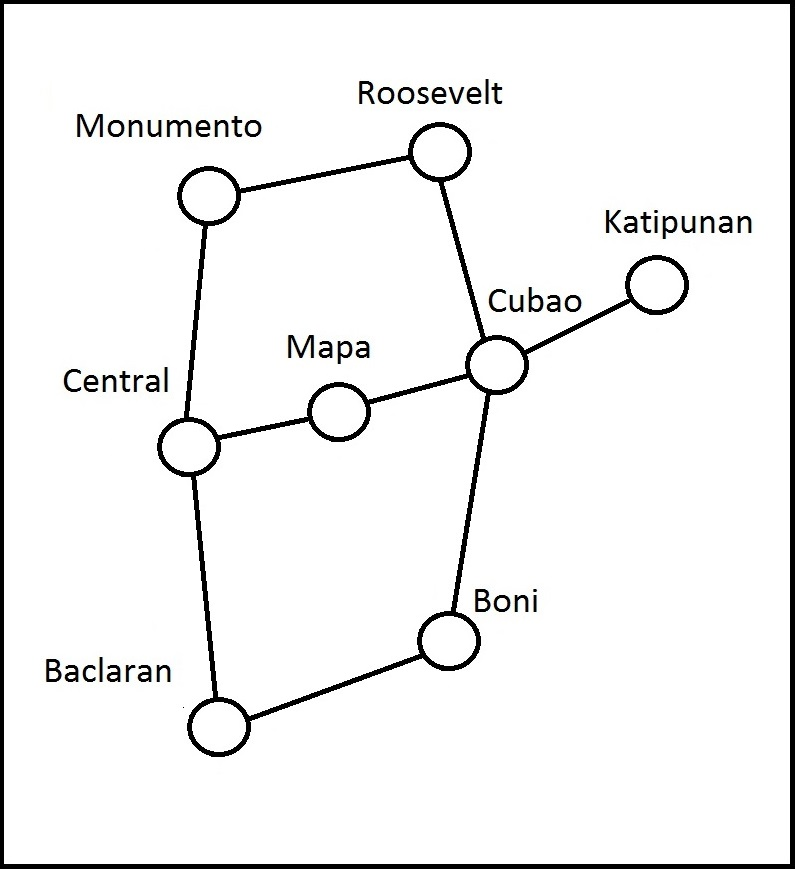
\includegraphics[width=\textwidth]{Manila-model_2}
\caption{The graph representing the connectivity of the city.}
\label{fig:map model}
\end{subfigure}
\caption{Modeling the map of Manila}
\label{fig:Manila}
\end{figure}

In the Agent-based model, the population is equally distributed in all of the nodes (areas) of the city. We consider that the city consists of home, work, public and leisure places. All of these kinds of places are also equally distributed throughout the city. In order for a person to be able to infect other people, all of those persons need to be located in the same place.% (home or work place, public or leisure place).

Each of those places has its own capacity and, thus, its own density, which also depends on the number of people that is currently in that place. Consequently, the probability of getting infected at time $t$ in the place $k$ is going to be equal to $$p_k(t) = d_k(t) \times i_k(t) \times \beta.$$ Where
\begin{itemize}
\item $d_k(t)$: density of the place $k$ which is equal to $\frac{\#\text{people in place }k}{\text{total capacity}}$ at time $t$,
\item $i_k(t)$: percentage of infected people which is equal to $\frac{\#\text{infected people in }k}{\#\text{people in }k}$ at time $t$, and
\item $\beta$: rate at which a person who has been exposed to the virus becomes infected, $0.9$. \textcolor{red}{Can we define that as $\beta$ instead of $a$?? Just to be consistent with the SEIR model}
\end{itemize}
 
\subsection{Population dynamics}
The daily activities of each agent can be briefly described using the following finite-state machine in Figure \ref{states}. 

\begin{figure}[H]
\centering
\xymatrix{*+<1pc>[][F-]{Resting} \ar[r] & *+<1pc>[][F-]{Commuting} \ar[r] & *+<1pc>[][F-]{Working} \ar[r] & *+<1pc>[][F-]{Commuting} \ar@{-->}[r]^p \ar@(u,u)@{-->}[lll]_{1-p} & *+<1pc>[][F-]{Leisure} \ar[r] & *+<1pc>[][F-]{Commuting} \ar@(d,d)[lllll] \\ *+<0.5pc>[][]{}}
\caption{States}
\label{states}
\end{figure}
Every agent has its own activity hours (or schedule) which means that each agent may spend different total time of hours in each activity. For example, a person may be working in a full-time job ($7$ hours), but another person may be working in a part-time job ($3$-$4$ hours). Therefore, we randomly set the activity hours of each agent using some distributions. 

For the total hours of work, a Gaussian distribution of $\mathcal{N}(7,2)$ is used. Correspondingly for the total hours of sleep, we use a Gaussian distribution of $\mathcal{N}(7,1)$. Moreover, we randomly set the place at which each agent works and rests. Depending on where the homeplace and the workplace of the agent is, the agent is going to spend a different span of time in commuting. 

Furthermore, a decision of having leisure time or not is made for each agent upon the beginning of the day. Every agent has its own probability of how often it decides to have leisure time. This probability is also distributed as a Gaussian with $\mathcal{N}(0.4,0.1)$. To define how much time the agent spends on commuting, we compute the distance from the source to the wanted destination using the Dijkstra's algorithm (as the map is represented as a graph of nodes). So, when the agent wants to move to another place (either for work, leisure or going back to home), is going to spend some time on commuting.

The step size of the simulation is one hour.

%% RESULTS
\section{Results}
We can analyse how will the virus spread among the population studying the variation of the amount of people who is in each state (S, E, I or R). So as to do at, we define a population of $10,000$ people where there is a person exposed. In addition, we use an infectious rate, $\beta$, of $0.9$, based on real data. We can see the result of that in the Figure \ref{agent_120_mean_data}. That figure is the averaged behaviour of $100$ iterations of the Agent-based model.

\subsection{Results}
We can analise how will the virus spreads among the population studying the variation of the amount of people who is in each state. So as to do at, we define a population of $10,000$ people where there is a person exposed. In addition, we use an infectious rate of $0.9$, based on real data. We can see the result of that in the Figure \ref{agent_120_1}.

 %% AB results
\begin{figure}[H] 
 \centering
 \begin{tikzpicture}
 \begin{axis}[legend pos = outer north east]
 \addplot[color=blue,mark=none] table [x expr=\thisrowno{0}, y expr=\thisrowno{1}, col sep=space] {data/agent_sim_120_1.txt};
\addlegendentry{Susceptible}
 \addplot[color=orange,mark=none] table [x expr=\thisrowno{0}, y expr=\thisrowno{2}, col sep=space] {data/agent_sim_120_1.txt};
 \addlegendentry{Exposed}
 \addplot[color=red,mark=none] table [x expr=\thisrowno{0}, y expr=\thisrowno{3}, col sep=space] {data/agent_sim_120_1.txt};
 \addlegendentry{Infectious}
 \addplot[color=green,mark=none] table [x expr=\thisrowno{0}, y expr=\thisrowno{4}, col sep=space] {data/agent_sim_120_1.txt};
 \addlegendentry{Recovered}
 \end{axis}
\end{tikzpicture}
 \caption{Results of the agent-based model}
 \label{agent_120_1}
 \end{figure}

As we can see in the Figure \ref{agent_120_mean_data}, the Measles virus needs around $30$ days to spread among other people. $30$ days after, it has expanded among all the population. We can see that observing that the number of susceptible people around the $60th$ day is closer to $0$. After that, the exposed people become infected and, little by little, all of them get recovered.

\subsection{The effects of infectious rate and the amount of initial exposed persons} % Variation of parameters
As we have said in the introduction, Measles virus has an infectious rate between $0.75$ and $0.9$. And we have used $\beta = 0.9$ to build up the Agent-based model. In order to analyse the consequences of that chosing, we want to compare the variation of the amount of people in each state depending on the value of $\beta$. We can see the results in the Figures \ref{fig:effects beta on S}, \ref{fig:effects beta on E}, \ref{fig:effects beta on I} and \ref{fig:effects beta on R}. All of the figures show that both curves have the same tendency with slight differences.

In the Figure \ref{fig:effects beta on S}, the difference is that the curve corresponding to $\beta=0.75$ starts decreasing later, which is logic according to the lower contact rate. In the Figures \ref{fig:effects beta on E} and \ref{fig:effects beta on I}, we can see that the maximum achieved by the dashed curves is lower than the one achieved by the other curves. That is a consequence of the higher amount of days that the model with $\beta=0.75$ needs to expand among the population. In that model the spreading will be slower but, at the end, the entire population will have get infected and, at the appropiate time, recovered, see Figure \ref{fig:effects beta on R}.

 %% The effects of infectious rate on the different groups
 \begin{figure}[H]
 \begin{minipage}{0.5\textwidth}
 \centering
 \begin{tikzpicture}
 \begin{axis}[scaled ticks=false, tick label style={/pgf/number format/fixed}, xlabel = Days, ylabel = Population]
 \addplot[color=blue,mark=none] table [x expr=\thisrowno{0}, y expr=\thisrowno{1}, col sep=space] {data/agent_sim_120_1.txt};
 \addlegendentry{$\beta=0.9$}
 \addplot[color=blue,mark=none,dashed] table [x expr=\thisrowno{0}, y expr=\thisrowno{1}, col sep=space] {data/agent_sim_120_1_0.75.txt};
 \addlegendentry{$\beta=0.75$}
 \end{axis}
 \end{tikzpicture}
 \caption{The effects of $\beta$ on the susceptible group}
 \end{minipage} \hspace{5mm} \begin{minipage}{0.5\linewidth}
 \begin{tikzpicture}
 \begin{axis}[xlabel = Days]
 \addplot[color=orange,mark=none] table [x expr=\thisrowno{0}, y expr=\thisrowno{2}, col sep=space] {data/agent_sim_120_1.txt};
 \addlegendentry{$\beta=0.9$}
 \addplot[color=orange,mark=none,dashed] table [x expr=\thisrowno{0}, y expr=\thisrowno{2}, col sep=space] {data/agent_sim_120_1_0.75.txt};
 \addlegendentry{$\beta=0.75$}
 \end{axis}
 \end{tikzpicture}
 \caption{The effects of $\beta$ on the exposed group}
 \end{minipage}
 \end{figure}
 
Now, we are going to study the effects of the initial amount of exposed people\footnote{In this section we will refer to the amount of people in one state as the letter which define each state. In other words, when we say "the effects of the initial E on S" we want to say "the effects of the initial amount of exposed people on the susceptible group".}. We distinguish four cases and those depend on the configuration of the initial population. Each case contains $1$ exposed person, $100$, $500$ and $1,000$ exposed people, respectively. We analyse the states' variation depending on the initial E, analogously as the infectious rate study. We can see the results in Figures \ref{fig:effects E on S}, \ref{fig:effects E on E}, \ref{fig:effects E on I} and \ref{fig:effects E on R}. Here, all the curves in each figure show the same tendency. The more exposed people, the faster the virus spreads. Consequently, the more exposed people, the less days the virus needs to expand among the entire population. A curious fact is the behaviour of the model when there are $500$ exposed people at the beginning. We can note in Figure \ref{fig:effects E on E} and \ref{fig:effects E on I} that the virus does not spread as fast as we could expect. That conclusion is based on the lower maximum it achieves. \textcolor{red}{As the whole population goes through all the states in all the cases, we know that the area below all the curves is the same. So, if the maximum is lower, it means that the model takes more days to infect the entire population.} 
 
 \begin{figure}[H]
 \begin{minipage}{0.5\textwidth}
 \centering
 \begin{tikzpicture}
 \begin{axis}[legend pos = north west, xlabel = Days, ylabel = Population]
 \addplot[color=red,mark=none] table [x expr=\thisrowno{0}, y expr=\thisrowno{3}, col sep=space] {data/agent_sim_120_1.txt};
 \addlegendentry{$\beta=0.9$}
 \addplot[color=red,mark=none,dashed] table [x expr=\thisrowno{0}, y expr=\thisrowno{3}, col sep=space] {data/agent_sim_120_1_0.75.txt};
 \addlegendentry{$\beta=0.75$}
 \end{axis}
 \end{tikzpicture}
 \caption{The effects of $\beta$ on the infectious group}
 \end{minipage} \hspace{5mm} \begin{minipage}{0.5\linewidth}
 \begin{tikzpicture}
 \begin{axis}[scaled ticks=false, tick label style={/pgf/number format/fixed}, legend pos = north west, xlabel = Days,]
 \addplot[color=green,mark=none] table [x expr=\thisrowno{0}, y expr=\thisrowno{4}, col sep=space] {data/agent_sim_120_1.txt};
 \addlegendentry{$\beta=0.9$}
 \addplot[color=green,mark=none,dashed] table [x expr=\thisrowno{0}, y expr=\thisrowno{4}, col sep=space] {data/agent_sim_120_1_0.75.txt};
 \addlegendentry{$\beta=0.75$}
 \end{axis}
 \end{tikzpicture}
 \caption{The effects of $\beta$ on the recovered group}
 \end{minipage}
 \end{figure}

 %% The effects of the initial infectious persons
 \begin{figure}[H]
 \begin{minipage}{0.5\textwidth}
 \centering
 \begin{tikzpicture}
 \begin{axis}[scaled ticks=false, tick label style={/pgf/number format/fixed}, xlabel = Days, ylabel = Population]
 \addplot[color=orange,mark=none] table [x expr=\thisrowno{0}, y expr=\thisrowno{1}, col sep=space] {data/agent_sim_120_1.txt};
 \addlegendentry{1 person}
 \addplot[color=magenta,mark=none] table [x expr=\thisrowno{0}, y expr=\thisrowno{1}, col sep=space] {data/agent_sim_120_100.txt};
 \addlegendentry{100 people}
 \addplot[color=cyan,mark=none] table [x expr=\thisrowno{0}, y expr=\thisrowno{1}, col sep=space] {data/agent_sim_120_500.txt};
 \addlegendentry{500 people}
 \addplot[color=black,mark=none] table [x expr=\thisrowno{0}, y expr=\thisrowno{1}, col sep=space] {data/agent_sim_120_1000.txt};
 \addlegendentry{1000 people}
 \end{axis}
 \end{tikzpicture}
 \caption{The effects of the initial E on S}
 \end{minipage} \hspace{5mm} \begin{minipage}{0.5\linewidth}
 \begin{tikzpicture}
 \begin{axis}[xlabel = Days]
 \addplot[color=orange,mark=none] table [x expr=\thisrowno{0}, y expr=\thisrowno{2}, col sep=space] {data/agent_sim_120_1.txt};
 \addlegendentry{1 person}
 \addplot[color=magenta,mark=none] table [x expr=\thisrowno{0}, y expr=\thisrowno{2}, col sep=space] {data/agent_sim_120_100.txt};
 \addlegendentry{100 people}
 \addplot[color=cyan,mark=none] table [x expr=\thisrowno{0}, y expr=\thisrowno{2}, col sep=space] {data/agent_sim_120_500.txt};
 \addlegendentry{500 people}
 \addplot[color=black,mark=none] table [x expr=\thisrowno{0}, y expr=\thisrowno{2}, col sep=space] {data/agent_sim_120_1000.txt};
 \addlegendentry{1000 people}
 \end{axis}
 \end{tikzpicture}
 \caption{The effects of the initial E on E}
 \end{minipage}
 \end{figure}
 
 \begin{figure}[H]
 \begin{minipage}{0.5\textwidth}
 \centering
 \begin{tikzpicture}
 \begin{axis}[legend style={at={(1,0.5)}}, xlabel = Days, ylabel = Population]
 \addplot[color=orange,mark=none] table [x expr=\thisrowno{0}, y expr=\thisrowno{3}, col sep=space] {data/agent_sim_120_1.txt};
 \addlegendentry{1 person}
 \addplot[color=magenta,mark=none] table [x expr=\thisrowno{0}, y expr=\thisrowno{3}, col sep=space] {data/agent_sim_120_100.txt};
 \addlegendentry{100 people}
 \addplot[color=cyan,mark=none] table [x expr=\thisrowno{0}, y expr=\thisrowno{3}, col sep=space] {data/agent_sim_120_500.txt};
 \addlegendentry{500 people}
 \addplot[color=black,mark=none] table [x expr=\thisrowno{0}, y expr=\thisrowno{3}, col sep=space] {data/agent_sim_120_1000.txt};
 \addlegendentry{1000 people}
 \end{axis}
 \end{tikzpicture}
 \caption{The effects of the initial E on I}
 \end{minipage} \hspace{5mm} \begin{minipage}{0.5\linewidth}
 \begin{tikzpicture}
 \begin{axis}[scaled ticks=false, tick label style={/pgf/number format/fixed}, legend style={at={(1,0.5)}}, xlabel = Days]
 \addplot[color=orange,mark=none] table [x expr=\thisrowno{0}, y expr=\thisrowno{4}, col sep=space] {data/agent_sim_120_1.txt};
 \addlegendentry{1 person}
 \addplot[color=magenta,mark=none] table [x expr=\thisrowno{0}, y expr=\thisrowno{4}, col sep=space] {data/agent_sim_120_100.txt};
 \addlegendentry{100 people}
 \addplot[color=cyan,mark=none] table [x expr=\thisrowno{0}, y expr=\thisrowno{4}, col sep=space] {data/agent_sim_120_500.txt};
 \addlegendentry{500 people}
 \addplot[color=black,mark=none] table [x expr=\thisrowno{0}, y expr=\thisrowno{4}, col sep=space] {data/agent_sim_120_1000.txt};
 \addlegendentry{1000 people}
 \end{axis}
 \end{tikzpicture}
 \caption{The effects of the initial E on R}
 \end{minipage}
 \end{figure}
 

% COMPARISON OF THE MODELS
\section{Comparison of the models}
It is difficult to validate this kind of model because we do not have enough field data. Therefore, we use a validated model to do it: an ODE model. The model that best approaches our model is the SEIR model.

% %% AB vs SEIR model
 \begin{figure}[H] \centering
\begin{tikzpicture}
\begin{axis}[scaled ticks=false, tick label style={/pgf/number format/fixed}, legend pos = outer north east, xlabel = Days, ylabel = Population]
\addplot[color=blue,mark=none,dashed] table [x expr=\thisrowno{0}, y expr=\thisrowno{1}, col sep=space] {data/agent_sim_120_1.txt};
\addlegendentry{Susceptible (Agent)}
\addplot[color=orange,mark=none,dashed] table [x expr=\thisrowno{0}, y expr=\thisrowno{2}, col sep=space] {data/agent_sim_120_1.txt};
\addlegendentry{Exposed (Agent)}
 \addplot[color=red,mark=none,dashed] table [x expr=\thisrowno{0}, y expr=\thisrowno{3}, col sep=space] {data/agent_sim_120_1.txt};
 \addlegendentry{Infectious (Agent)}
 \addplot[color=green,mark=none,dashed] table [x expr=\thisrowno{0}, y expr=\thisrowno{4}, col sep=space] {data/agent_sim_120_1.txt};
 \addlegendentry{Recovered (Agent)}
 \addplot[color=blue,mark=none] table [x expr=\thisrowno{0}, y expr=\thisrowno{1}, col sep=space] {data/seir_data_120_1.txt};
 \addlegendentry{Susceptible (SEIR)}
 \addplot[color=orange,mark=none] table [x expr=\thisrowno{0}, y expr=\thisrowno{2}, col sep=space] {data/seir_data_120_1.txt};
\addlegendentry{Exposed (SEIR)}
 \addplot[color=red,mark=none] table [x expr=\thisrowno{0}, y expr=\thisrowno{3}, col sep=space] {data/seir_data_120_1.txt};
 \addlegendentry{Infectious (SEIR)}
 \addplot[color=green,mark=none] table [x expr=\thisrowno{0}, y expr=\thisrowno{4}, col sep=space] {data/seir_data_120_1.txt};
 \addlegendentry{Recovered (SEIR)}
 \end{axis}
 \end{tikzpicture}
 \caption{Comparison of the agent-based model with the SEIR model}
 \end{figure}




%% CONCLUSION
\section{Conclusion}
- Possibly also future work

%% REFERENCES
\bibliographystyle{plain}
\addcontentsline{toc}{section}{References}
\bibliography{bibliography.bib}

%% APPENDIX
\section{Appendix}

\end{document}